L\textquoteright{}Organizational Breakdown Structure, abbreviata in OBS, \`{e} una scomposizione gerarchica delle responsabilit\`{a} che rappresenta l\textquoteright{}organizzazione del progetto. Viene generata allo scopo di individuare univocamente i responsabili o gli esecutori dei WP e migliorare il fusso di comunicazioni del progetto. Il diagramma che segue ha lo scopo di identificare chiaramente i ruoli principali all\textquoteright{}interno del progetto.

\begin{figure}[H]
\centering % per centrare l'immagine (opzionale)
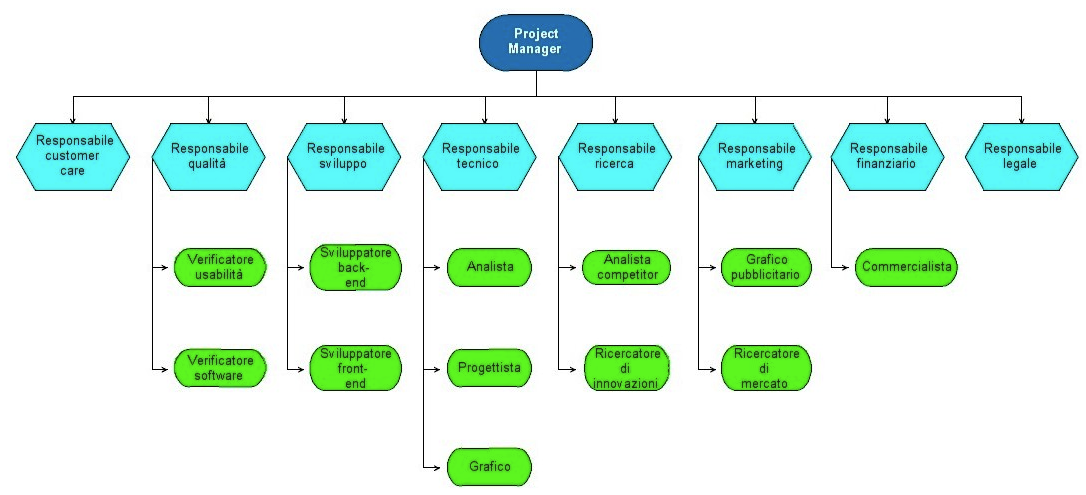
\includegraphics[scale=0.4]{img/Progetto2.png}
\caption{Diagramma OBS}
\label{fig:Diagramma OBS}
\end{figure}

\subsubsection{Project manager}
Responsabile ultimo del completamento del progetto, i suoi obblighi comprendono:
\begin{itemize}
\item realizzazione del progetto nel rispetto dei requisiti funzionali, di qualit\`{a} e dei
vincoli imposti;
\item rispetto dei tempi di consegna e dei costi preventivati;
\item rispetto dei margini di profitto preventivati.
Per assicurarsi di far fronte ai suoi obblighi, il PM pianifica tutte le fasi del progetto
coordinando le risorse per assicurare il conseguimento degli obbiettivi, anche in caso di
circostanze inaspettate.
\end{itemize}

\subsubsection{Responsabile customer care}
Il RCC deve:
\begin{itemize}
\item scegliere le modalit\`{a} con cui gli utenti possono comunicare all\textquoteright{}azienda;
\item scegliere i servizi a cui appoggiarsi per gestire il rapporto con i clienti;
\item intrattenere rapporti diretti con i clienti pi\`{u} importanti, eventualmente con il
supporto del PM;
\item stendere rapporti mensili (da consegnare al PM) inerenti le maggiori problematiche
riscontrate dai clienti o con i mezzi di comunicazione e i servizi adottati.
\end{itemize}

\subsubsection{Responsabile qualit\`{a}}
Il RQ ha il compito di definire gli standard di qualit\`{a} da rispettare per ogni singolo processo
svolto dall\textquoteright{}azienda e di promuovere il miglioramento dei processi in corso di sviluppo.
Si attiene strettamente alle normative in materia di qualit\`{a} (ISO 9000/9001/9004
e ISO 9126 relativamente alla qualit\`{a} del software) e, a seguito dell\textquoteright{}analisi dei singoli
processi, promuove azioni di miglioramento, sia attraverso comunicazioni interne all\textquoteright{}azienda,
che attraverso formazione specifica degli addetti. Il miglioramento continuo
della qualit\`{a} aziendale, seguendo le linee guida del CMMI\footnote{Capability Maturity Model Integration - \url{http://it.wikipedia.org/wiki/Capability\_Maturity\_Model}}, garantisce all\textquoteright{}azienda un
miglioramento dell\textquoteright{}efficienza ed una maggiore soddisfazione dei clienti. Per quanto riguarda
il prodotto software sviluppato, il RQ deve inoltre comunicare al PM i verbali
ottenuti dai suoi sottoposti e proporre attivit\`{a} mirate all\textquoteright{}incremento della qualit\`{a}.

\subsubsection{Verificatore usabilit\`{a}}
L\textquoteright{}azienda crede fermamente che un prodotto altamente usabile (vedi ISO 9241) sia
sinonimo di qualit\`{a} e sia in parte garanzia di successo. Per questo motivo, contemporaneamente
alla verifica di accessibilit\`{a} del prodotto, il verificatore valuter\`{a} eventuali
migliorie sul piano dell\textquoteright{}usabilit\`{a} e rediger\`{a} un verbale per il RQ esponendo le eventuali problematiche riscontrate e le possibili soluzioni.

\subsubsection{Verificatore software}
Tra le varie fasi che compongono la creazione di un prodotto software, c\textquoteright{}\`{e} il testing.
Questa operazione viene svolta dagli sviluppatori (SF e SB) e punta all\textquoteright{}eliminazione del
maggior numero di bug possibili. Una fase altrettanto importante \`{e} quella della verifica
e della validazione del software (vedi IEEE 1012), in questo caso il VS deve controllare
che quanto prodotto rispetti i requisiti espressi nel documento di Analisi dei Requisiti
redatto dall\textquoteright{}analista e sia effettivamente quanto richiesto. Al termine di ogni sessione di verifica il VS rediger\`{a} un verbale per il RQ.

\subsubsection{Responsabile tecnico}
Il RT coordina ogni fase dello sviluppo dei prodotti software dell\textquoteright{}azienda ed \`{e} il responsabile
dello stato di avanzamento dei prodotti nel rispetto delle scadenze temporali e
dei costi. Ha una competenza tecnica molto vasta e deve potersi
relazionare con i suoi subordinati su ogni aspetto dello sviluppo.\\
Una volta ricevuto l\textquoteright{}incarico dal PM:
\begin{enumerate}
\item assegna all\textquoteright{}analista il compito di formalizzare quanto dev\textquoteright{}essere prodotto;
\item al termine della fase di analisi, incarica:
\begin{itemize}
\item il Progettista di delineare l\textquoteright{}architettura di dettaglio;
\item il Grafico di stendere le bozze delle interfacce utente.
\end{itemize}
\item durante la fase di progettazione, il RT controlla che l\textquoteright{}architettura software rispetti
le metriche software concordate e propone al progettista eventuali modifiche. Nel
caso fosse necessario (utilizzo di un nuovo linguaggio/framework), predispone corsi
di aggiornamento o di formazione per gli sviluppatori;
\item al termine della fase di progettazione, consegna quanto prodotto al RS;
\item coordina le operazioni di manutenzione successive al rilascio.
\end{enumerate}

\subsubsection{Analista}
L\textquoteright{}analista ha il compito di formalizzare quanto emerso dalle discussioni con il PM e
dalla lettura della documentazione di presentazione del progetto. Redige lo "Studio di Fattibilit\`{a}", nel quale si indica se il progetto \`{e} fattibile e quali sono le aree critiche ed il documento di Analisi dei Requisiti nel quale, con l\textquoteright{}ausilio di diagrammi dei casi d\textquoteright{}uso e di altri formalismi(vedi INCOSE\footnote{International Council on Systems Engineering - \url{http://www.incose.org/}}), viene riportato cosa sar\`{a} sviluppato. Al termine della fase di analisi l\textquoteright{}analista consegner\`{a} entrambi i documenti al RT.

\subsubsection{Progettista}
La fase di progettazione ha inizio con la delibera, da parte del PM, di quanto prodotto
dall\textquoteright{}analista e con la conseguente assegnazione dell\textquoteright{}incarico al Progettista. Una volta
studiata l\textquoteright{}Analisi dei Requisiti, il progettista redige dapprima il documento di "Specifica
Tecnica", nel quale viene proposta una soluzione ad alto livello del problema focalizzandosi
maggiormente sulle funzionalit\`{a}, piuttosto che sulla loro implementazione, e successivamente
il documento di "Definizione di Prodotto" nel quale si propone una soluzione concreta e
dettagliata al problema posto. In entrambi i documenti il progettista far\`{a} ampio uso di
diagrammi e schemi per rendere il pi\`{u} chiara possibile qualsiasi scelta implementativa.
Al termine della fasi di progettazione i documenti prodotti sono consegnati al RT.

\subsubsection{Grafico}
Il grafico viene incaricato dal RT di creare le bozze per ogni interfaccia utente presente
nel progetto. Il lavoro inizia con la lettura dell\textquoteright{}"Analisi dei Requisiti" e, in particolare,
con la sezione relativa ai casi d\textquoteright{}uso che indicano, tra l\textquoteright{}altro, quante possibili bozze sono
necessarie. Una volta create, le bozze vengono consegnate al PM che le valuta con
l\textquoteright{}ausilio del team del RQ e, se necessario, con il RDM.

\subsubsection{Responsabile sviluppo}
Il RS coordina ogni fase dello sviluppo dei prodotti software dell\textquoteright{}azienda ed \`{e} il responsabile
dello stato di avanzamento dei prodotti nel rispetto delle scadenze temporali e
dei costi. Ha una competenza tecnica molto vasta assimilata e deve potersi
relazionare con i suoi subordinati su ogni aspetto dello sviluppo. Una volta ricevuto
l\textquoteright{}incarico dal RT in accordo con il PM:
\begin{itemize}
\item suddivide gli incarichi di lavoro tra SF e SB in base a quanto fornito dal RT;
\item durante la fasi di sviluppo, segue attentamente i report relativi ai test effettuati e
controlla lo stato di avanzamento del prodotto in relazione alle scadenze prefissate;
\item supervisiona le fasi di alpha e beta testing ed i successivi test di collaudo precedenti
il rilascio.
\end{itemize}

\subsubsection{Sviluppatore front-end}
Lo SF viene incaricato dal RS di realizzare e successivamente manutenere tutte le parti
software con cui interagisce l\textquoteright{}utente, oltre ai documenti tecnici prodotti dal Progettista
gli vengono consegnate anche le bozze create dal Grafico.

\subsubsection{Sviluppatore back-end}
Lo SB viene incaricato dal RS di realizzare e successivamente manutenere tutte le parti
software che elaborano dati e non sono a diretto contatto con l\textquoteright{}utente, per svolgere il
suo compito necessita solo dei documenti tecnici prodotti dal Progettista.

\subsubsection{Responsabile ricerca}
Il mercato attuale \`{e} in continua evoluzione ed anche potendo contare su un prodotto
di successo, bisogna essere in grado di migliorarlo continuamente per poter rimanere al
passo rispetto alla concorrenza. Il RR quindi coordina il suo team per:
\begin{itemize}
\item rimanere al passo con i competitor, analizzando le funzionalit\`{a} da loro
implementate e capendo quali di esse potrebbero dare un valore aggiunto al
progetto;
\item creare un gap rispetto ai competitor, cercando soluzioni innovative non ancora
presenti sul mercato e che facciano evolvere positivamente il progetto.
\end{itemize}

\subsubsection{Analista competitor}
L\textquoteright{}AC deve scandagliare tutti i "rivali" del prodotto che si sta sviluppando e cercare
di capire quali delle soluzioni da loro implementate possano dare un tangibile valore
aggiunto al progetto. A ricerca completata l\textquoteright{}AC produrr\`{a} una documentazione di quanto
trovato e la consegner\`{a} per valutazione al RR.

\subsubsection{Ricercatore di innovazioni}
Il RI basandosi su quanto reso disponibile dal prodotto e su eventuali trend di mercato
in settori affini, cerca di trovare novit\`{a} da poter implementare nel prodotto al fine di
aumentare: le funzionalit\`{a} offerte, la soddisfazione dell\textquoteright{}utente, il bacino di utenza e di
estendere eventualmente il target del prodotto. Al termine del processo il RI produrr\`{a}
una documentazione che sar\`{a} consegnata per valutazione al RR.

\subsubsection{Responsabile marketing}
Il RM ha l\textquoteright{}onere di posizionare i prodotti nel mercato di riferimento e di renderli profittevoli.
Per adempiere al suo compito analizza il mercato individuando cos\`{i} le opportunit\`{a}
di business e progetta ed attua le strategie di marketing pi\`{u} efficaci per l\textquoteright{}incremento
dei profitti e per l\textquoteright{}affermazione del brand.

\subsubsection{Grafico Pubblicitario}
Per far conoscere l\textquoteright{}azienda ai possibili utilizzatori e per stimolare l\textquoteright{}adozione dei prodotti
proposti \`{e} indispensabile avere campagne pubblicitarie efficaci. Il GP, sotto la
supervisione del RM, crea le pubblicit\`{a} dell\textquoteright{}azienda.

\subsubsection{Ricercatore di mercato}
Il RDM ha competenze statistiche specifiche nella creazione di sondaggi e nell\textquoteright{}analisi
dei dati ottenuti; ha lo scopo di comprendere qual \`{e} l\textquoteright{}opinione delle persone relativamente
all\textquoteright{}azienda e ai prodotti da essa sviluppati e quali sono, in generale, gli aspetti
migliorabili. Si occupa, quindi, di redigere sondaggi ai fini di comprendere:
\begin{itemize}
\item qual \`{e} il target di riferimento;
\item quanto gli utenti conoscono i prodotti sviluppati dall\textquoteright{}azienda;
\item il livello di qualit\`{a} e seriet\`{a} che gli utenti attribuiscono all\textquoteright{}azienda e ai suoi
prodotti;
\item eventuali aspetti negativi riscontrati o miglioramenti proposti.
\end{itemize}

\subsubsection{Responsabile finanziario}
Il RF ha il compito di monitorare il flusso di cassa dell\textquoteright{}azienda e di individuare eventuali
problematiche ben prima che si verifichino. Si avvale di un Commercialista per le
operazioni contabili e di un BF per massimizzare le rendite dell\textquoteright{}azienda.

\subsubsection{Commercialista}
Il Commercialista \`{e} incaricato dall\textquoteright{}azienda di mantenerne la contabilit\`{a}, di effettuare i
versamenti delle tasse e di verificare e legittimarne le operazioni economiche.

\subsubsection{Responsabile legale}
Il RL viene contattato dall\textquoteright{}azienda quando:
\begin{itemize}
\item si vuole garantire che i software sviluppati rispettino le normative vigenti, nello
specifico quelle relative alla privacy;
\item si vogliono archiviare particolari brevetti o si vuole garantire il copyright di un
prodotto;
\item nascono dispute legali tra terzi e l\textquoteright{}azienda;
\item si sviluppano trattative economiche delle quali non \`{e} del tutto chiara la legittimit\`{a}.
\end{itemize}
